\documentclass[a4paper,12pt]{report}


\usepackage[utf8]{inputenc}		% Accents, etc
\usepackage[frenchb]{babel} 		% Francais
\usepackage[T1]{fontenc}			% Encodage de police (césure, accents)
\usepackage{lmodern,textcomp}	% Polices 'Latin Modern' plutôt que 'Computer Modern super'

\usepackage[pdftex]{graphicx}			% Graphiques (images, ...)
\usepackage{amsmath,amssymb}		% Equations
\usepackage[pdftex]{hyperref}	% Lien table des matières

\usepackage[squaren,Gray]{SIunits}

\usepackage{titlesec}			% Chapitres
\titleformat{\chapter}[hang]{\bf\huge}{\thechapter}{2pc}{}

% Symbole euro €
\usepackage{eurosym}

% Floating figures
\usepackage{wrapfig}

% Subfigures
\usepackage{subfig}

% Marges du document
\usepackage{geometry}
\geometry{top=2cm, bottom=2cm, left=25mm, right=25mm}

%
\usepackage{rotating}

% Taille des sous-titres
%\usepackage{titlesec}
%\titleformat{\subsection}{\small\bfseries}{\thesection}{1em}{}

% Page de titre du document
\title{Projets de groupe \\ Rapport Final}
%\author{J. \bsc{Fanguede}, F. \bsc{Castellane}, G. \bsc{Mahieux}, F. \bsc{Tavares}}
\author{\bsc{F. Castellane} \and \bsc{J. Fanguede} \and \bsc{G. Mahieux} \and \bsc{F. Tavares}  }
\date{Février 2012}

% Réglages des métadata du PDF
\hypersetup{
pdftitle={Rapport Final},
pdfauthor={F. Castellane, J. Fanguede, G. Mahieux, F. Tavares},
pdfsubject={Projets de groupe 2012},
pdfkeywords={Phelma, Projet, Grenoble, INP, Flyport, OpenPicus, WiFi}
}
% Ligne horizontale
\newcommand{\HRule}{\rule{\linewidth}{0.5mm}}


% Début du document
\begin{document}

\setlength{\parskip}{1ex plus 0.5ex minus 0.2ex}

\begin{titlepage}
	\begin{center}
	
	% Upper part of the page
	
\includegraphics[width=0.25\textwidth]{images/smallphelma.png}\\[1.0cm]    

	\textsc{\Large Grenoble INP -- Phelma}\\[0.5cm]

	\textsc{\huge Projet de groupe}\\[3.5cm]

	\textsc{\huge Voiture Radiocommandée en Wi-Fi}\\[0.6cm]
	
	% Title
	\HRule \\[0.4cm]
	{ \huge \bfseries Rapport Final}\\[0.1cm]

	\HRule \\[3.5cm]
	

	% Author and supervisor
	\begin{minipage}{0.3\textwidth}
		\begin{flushleft} \large
			\emph{Groupe:}\\
			Florian \textsc{Castellane}, \\ Jérémy \textsc{Fanguède}, \\ Guillaume \textsc{Mahieux}, \\ Florian \textsc{Tavares}
		\end{flushleft}
	\end{minipage}
	\begin{minipage}{0.4\textwidth}
		\begin{flushright} \large
			\emph{Tuteur:} \\
			Sylvain \textsc{Huet}
		\end{flushright}
	\end{minipage}
	\vfill

% Bottom of the page
{\large \today}

\end{center}

\end{titlepage}

% Page de titre du document
%\maketitle

% Remerciements
\chapter*{Remerciements}
Tout d’abord, nous souhaitons remercier notre tuteur de projet, M. Huet, pour l’aide et le regard critique qu’il nous a apporté dans le choix de certaines solutions techniques du projet, ainsi que tout l’équipe encadrante des projets à Phelma pour leur accompagnement et leur aide quand à l’utilisation et le prêt de matériel de l’école. On pense tout particulièrement à Kamel Mahfoudhi, Sophie Cornu, Patrice Petitclair et Laurent Aubard pour leurs conseils en matière d’électronique et Antoine Pisa pour sa réactivité dans la réalisation des circuits imprimés (commandés à 10h, reçus à midi !).

Nous voulons également remercier l’entreprise \emph{OpenPICUS} pour avoir soutenu notre démarche en offrant un module \emph{OpenPICUS Flyport ®} à Phelma pour mener à bien notre projet, ainsi que \emph{STMicroelectronics} pour nous avoir envoyé deux contrôleurs de moteurs \emph{L298} via leur programme \emph{free samples}.

% Introduction
\chapter*{Introduction}
Le projets de groupe occupe une place importante du programme pédagogique
de première année à Phelma. Il permet aux étudiants de se familiariser avec la gestion de projet, une des composantes essentielles du métier d’ingénieur.
On distingue deux types projets distincts avec chacun leur avantages et leurs inconvénients : 
\begin{itemize}
	\item ceux à vocation sociale
	\item ceux à vocation technique
\end{itemize}
Les premiers permettent notamment de développer des compétences humaines indissociables du métier d’ingénieur dans ce monde mondialisé. Les seconds permettent de perfectionner la compréhension de systèmes de nature complexe, rôle historique de l’ingénieur.
L’idéal aurait été d’aborder les deux. Malheureusement, nous avons été contraint de faire un choix. Nous avons décidé de retenir un sujet de nature technique dont l’intitulé est : “Voiture radio-commandée Wi-Fi”.

Concrètement, l’objectif de ce projet est de concevoir le système de commande d’un modèle réduit de voiture, ceci incluant aussi bien l’électronique embarquée que le logiciel de contrôle à distance du véhicule. Ce projet de robotique a principalement attiré notre attention du fait de sa pluridisciplinarité. En effet, la réalisation d’un tel système implique des compétences à la fois en électronique et en informatique, matières sur lesquelles tous les membres du groupe partagent un intérêt commun. Même si  la norme Wi-Fi tend à se banaliser de nos jours, son utilisation pour ce type d’application précis peut, dans un premier temps, surprendre. En effet, une connexion Wi-Fi est plus compliquée à mettre en œuvre, plus chère et plus consommatrice qu’une liaison RF maître-esclave habituellement utilisée dans ce type de systèmes. Cependant, l’avantage du Wi-Fi est que, une fois implémenté, il offre une couche d’abstraction logicielle de haut niveau permettant des communications à double sens entre le contrôleur et la machine à contrôler. Ainsi, il est tout à fait possible d’imaginer de faire remonter des informations obtenues à l’aide de capteurs installés sur le véhicule jusqu’au contrôleur sans modification particulière sur le matériel.

Sur la forme, ce rapport se découpe en deux parties traitant respectivement de la réalisation technique du dispositif et de la gestion du projet. Ces deux parties sont intentionnellement de tailles inégales, ceci pour rester en accord avec la consigne. Le rapport technique se veut abordable par le plus grand nombre et de difficulté croissante. Afin de faciliter la compréhension, nous avons jugé bon de rappeler le rôle et le principe de fonctionnement de chacune des solutions déployées avant de vous exposer notre réalisation. 

% Table des matières
\tableofcontents

% Début du document
\chapter{Rapport technique}

	\section{Cahier des charges}
	Le système à réaliser devait comporter un certain nombre de fonctionnalités obligatoires à son bon fonctionnement. En particulier, pouvoir contrôler le véhicule d’une manière relativement fluide, offrir une interface de contrôle sur une plate-forme adaptée et disposer d’une autonomie d’au moins quelques minutes. Ce cahier des charges est décrit sur la figure~\ref{cahierdescharges}. Des améliorations étaient prévues, notamment l’ajout de capteurs divers, bien que l’avancement du projet ne nous ait pas permis de tout mettre en oeuvre.
	
\begin{figure}%[!h]
	\begin{enumerate}
		\item Voiture radio-commandée
		\begin{enumerate}
    			\item Système de connectivité sans-fil
				\begin{enumerate}
    					\item Norme Wi-Fi IEEE 802.11 B/G/N
    					\item Protocoles de communication standards (ex: TCP / IP)
  				\end{enumerate}
    			\item Être contrôlable par un protocole interne
				\begin{enumerate}
    					\item Syntaxe des commandes
  				\end{enumerate}
			\item Rouler à une vitesse satisfaisante
			\item Avoir une autonomie suffisante
    			\item Offrir un retour d’informations au client
				\begin{enumerate}
    					\item Niveau de batterie
					\item Capteurs de proximité
					\item Caméra vidéo
  				\end{enumerate}
  		\end{enumerate}

		\item Logiciel de télécommande
		\begin{enumerate}
    			\item Être implémentable facilement sur une grande variété de plates-formes
				\begin{enumerate}
    					\item Utilisation de protocoles de communication standards (voir 1.a.ii)
  				\end{enumerate}
    			\item Offrir une interface utilisateur conviviale et fonctionnelle
				\begin{enumerate}
    					\item Contrôles adaptés à la plate-forme (ordinateur, smartphone)
  				\end{enumerate}
			\item Pouvoir afficher certaines grandeurs en temps réel (voir 1)
  		\end{enumerate}
	\end{enumerate}

	\caption{Cahier des charges fonctionnel}
	\label{cahierdescharges}
\end{figure}


	\section{Schéma fonctionnel}
	En accord avec le cahier des charges, la figure~\ref{schemafonctionnel} présente rapidement les différentes composantes de l’ensemble et leurs interactions. Celui-ci est composé de deux entités : la télécommande et le véhicule.
La télécommande correspond au logiciel de contrôle qui sera développé sur PC et smartphone. Celle-ci permettra de contrôler le véhicule et de régler certains paramètres.
La voiture devra disposer d’un module Wi-Fi et d’un circuit capable de contrôler les moteurs en fonction des commandes interprétées.

\begin{figure}%[!h]
	\begin{center}
		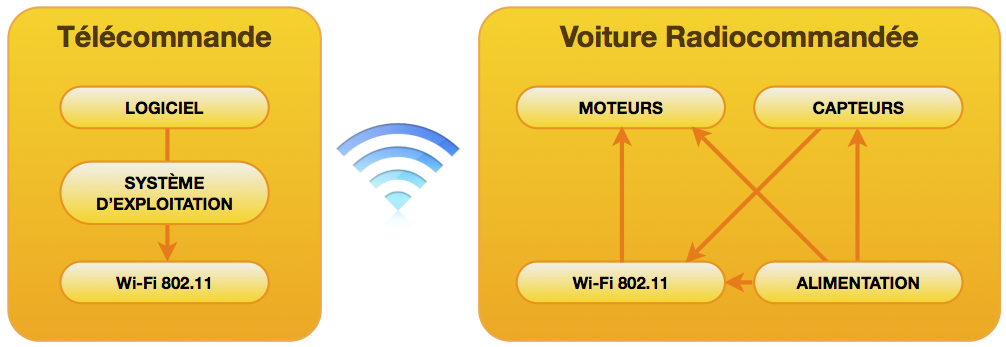
\includegraphics[scale=0.75]{images/schemafonctionnel.png}
	\end{center}
	\caption{Schéma fonctionnel du système} 
	\label{schemafonctionnel}
\end{figure}

	Nous avons découpé le système et analysé ce qu’il était nécessaire de faire, ainsi nous avons identifié un certain nombre de tâches à effectuer dans le cadre du projet. Celles-ci sont représentées sur le diagramme WBS en figure~\ref{wbs}.
	
	\begin{figure}%[!h]
	\begin{center}
		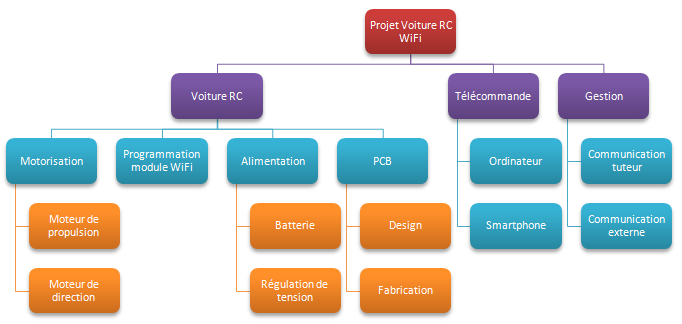
\includegraphics[scale=1.1]{images/wbs.png}
	\end{center}
	\caption{Diagramme WBS} 
	\label{wbs}
	\end{figure}
	
	\section{Solutions techniques à mettre en oeuvre}
	Cette section présente les différents organes du projet sans rentrer dans le détail de leur implantation. Elle explique leur intérêt et fonctionnement général.
	
		\subsection{Voiture}
		
			\subsubsection{Cadre}
			Le cadre est la partie qui sert de support aux différents composants (électroniques et mécaniques) de la voiture. Sa fonction principale est donc avant tout une fonction utilitaire. Toutefois, il peut devenir un élément de design lorsque qu’il reproduit avec fidélité le design de vraies voitures.
Pour ce projet, il convient d’utiliser un cadre conforme à la norme en matière de radiomodélisme, c’est-à-dire un cadre un plastique rigide. De cette façon, l’ensemble reste assez léger et peut donc être facilement animé par des moteurs à courant continu, tout en étant résistant aux chocs liés à l’utilisation du véhicule.
			
			\subsubsection{Servo-Moteur}
			Un servomoteur est un mécanisme qui effectue une rotation d’un axe en fonction d’une commande. Ce dispositif est nécessaire au contrôle de la direction de la voiture car il permet d’orienter les roues avant du véhicule grâce à un asservissement de position. Il est constitué:
\begin{itemize}
\item d’un moteur associé à un réducteur assurant la rotation de l’axe,
\item d’un capteur renvoyant une information relative à l’angle de l’axe,
\item d’une partie électronique qui gère le contrôle du moteur en fonction de la position fournie par la commande
\end{itemize}

Un servomoteur standard est composé de trois fils : deux pour l’alimentation (tension haute et basse) et un pour la commande. La position désirée est envoyée au servomoteur par l’intermédiaire de ce dernier fil sous la forme de signaux PWM (Pulse Width Modulation).
Un signal PWM est composé d’impulsions périodiques. La largeur de ces impulsions détermine la position voulue pour le servomoteur. En la changeant, il est donc possible de commander la direction de la voiture. La période des signaux PWM envoyée est généralement comprise entre 8 et 20 ms et la largeur de l’impulsion varie entre 0,7 et 2,3 ms. La figure~\ref{pwm} illustre ce mode de commande. Ces données varient toutefois selon les modèles de servomoteur et il convient de suivre les recommandations de chaque constructeur.

\begin{figure}%[!h]
	\begin{center}
		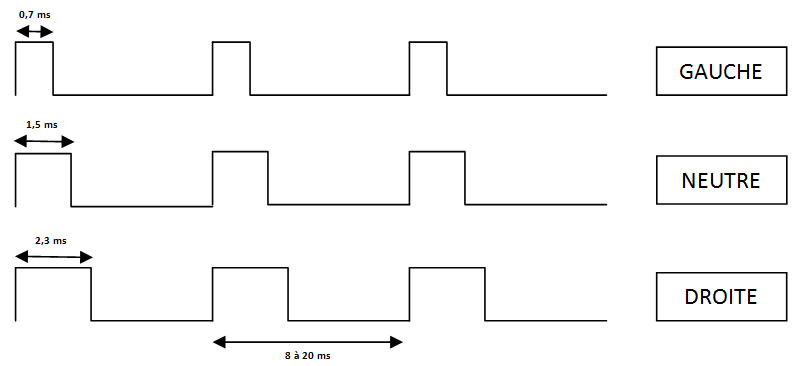
\includegraphics[scale=0.75]{images/pwm.png}
	\end{center}
	\caption{Principe de la commande à impulsions} 
	\label{pwm}
\end{figure}
			
			\subsubsection{Moteur de propulsion}
			Très utilisé en robotique et en modélisme, le moteur à courant courant continu (DC) est très simple à piloter. Il suffit de le brancher sur une alimentation avec une tension adéquate pour qu’il se mette à tourner. Le courant consommé dépend ensuite de la puissance à fournir, qui est évidement plus grande au démarrage ou lorsqu’on bloque la rotation.
			
			\subsubsection{Pont en H}
			Comme nous venons de le voir, contrôler un moteur à courant continu est une tâche relativement simple, il suffit de le brancher sur une alimentation adéquate. Ceci étant dit, quand il s’agit d’automatiser le fonctionnement du système, il n’est évidement pas question d’aller brancher et débrancher le moteur à la demande.
Pour activer le moteur, on utilise un montage de contrôle appelé pont en H (du fait de la forme de son schéma). Ce montage consiste en 4 interrupteurs placés de part et d’autre du moteur, entre celui-ci, l’alimentation et la masse. En activant ces interrupteurs d’une manière intelligente, on peux ainsi mettre chaque borne du moteur soit à la tension d’alimentation, soit à la masse. Il en résulte que l’on est capable de faire tourner le moteur dans les deux sens, ou de l’arrêter.
Les interrupteurs du pont peuvent être réalisés à l’aide de transistors ou de relais. Le  schéma de principe ci-dessous présente un pont en H à base de transistors bipolaires.

\begin{figure}%[!h]
	\begin{center}
		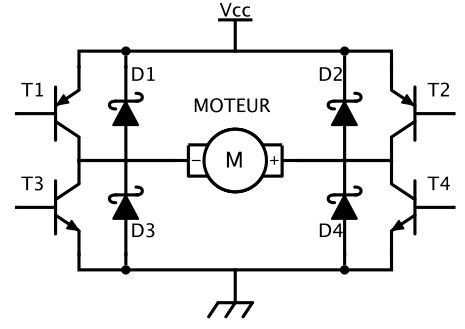
\includegraphics[scale=1]{images/hbridge.png}
	\end{center}
	\caption{Principe du \emph{pont en H}} 
	\label{hbridge}
\end{figure}

Nous souhaitons insister sur deux points :
\begin{itemize}
\item Il faut prendre soin de ne pas commuter les transistors T1/T3 et T2/T4 en même temps, car on pourrait avoir quelques instants pendant lesquels l’alimentation serait court-circuitée, ce qui pourrait endommager le système. On introduit un temps mort dans la commande pour résoudre ce problème.
\item Lorsqu’on commute le transistor, on force brutalement le courant à zéro, ce qui crée une surtension sur les transistors légèrement inductifs ($U = L*\partial{I}/\partial{t}$). Cette surtension est susceptible de détruire les transistors du pont, on utilise donc des diodes dites de roue libre pour absorber ce choc de courant et de tension.
\end{itemize}
			
			\subsubsection{Gestion du Wi-Fi}
			Pour être conforme au cahier des charges, notre voiture doit être conforme à la norme IEEE 802.11 B/G/N. Elle doit donc comporter un module Wi-Fi permettant de communiquer avec l’utilisateur par le biais de logiciels de commande. Deux critères importants sont à vérifier lors de notre choix final. D’une part, l’autonomie : en effet, le Wi-Fi est par nature un protocole de haut niveau et donc assez énergivore. Il convient de choisir un module fonctionnant sur batterie et ne consommant pas trop de courant. Le deuxième élément sur lequel il convient d’apporter une attention particulière est l’encombrement. Mettre un routeur Wi-Fi classique sur notre voiture est tout simplement hors de question, nous devons nous tourner vers des solutions dédiées à l’embarqué.
			
			\subsubsection{Micro-contrôleur}
			Un microcontrôleur est un circuit intégré qui rassemble les éléments essentiels d’un ordinateur: processeur, mémoire (Flash pour les programmes et RAM pour les données), interfaces entrées/sorties. Sa petite taille, sa faible consommation électrique et son coût réduit par rapport à un ordinateur classique en font un élément souvent retenu dans les systèmes embarqués.
Dans le cadre de notre projet, ce composant se chargera de récupérer les informations envoyées par le module de réception Wi-Fi, de les interpréter et de piloter les éléments mécaniques du véhicule (moteur et servomoteur) en conséquence.
			
		\subsection{Commande}
		Outre la réalisation de la voiture, il convient de mettre en place un dispositif permettant un contrôle à distance du véhicule. La norme Wi-Fi se généralisant de plus en plus, il est possible d’imaginer pléthore d’équipements pour commander la voiture : de l’ordinateur personnel aux smartphones (Android, iPhone)  en passant par les consoles de jeux portables.
Dans tous les cas, notre ou nos télécommandes seront programmées sur des systèmes disposant d’une interface Wi-Fi de haut niveau. De plus, celle-ci devra comporter une interface utilisateur de type graphique (GUI pour Graphical User Interface).
		
	\section{Réalisation technique}
	Cette section présente les choix qui ont étés retenus pour chaque bloc fonctionnel de la voiture, leur fonctionnement et les difficultés rencontrées avec leur utilisation.
	
		\subsection{Choix techniques retenus}
		
			\subsubsection{Châssis Nikko}
			Réaliser son propre cadre est une tache compliquée. Il faut prévoir des emplacements pour les moteurs, pour la batterie, créer un système de direction performant… D’autre part, on remarque que le coût total de toutes les pièces nécessaires à la réalisation d’un châssis maison dépasse souvent le prix d’une voiture télécommandée made in China.
Pour des raisons évidentes de coût et de charge de travail, nous avons donc décidé de baser notre travail sur un cadre de voiture existant : un modèle 1/10\ieme~de la marque Nikko d’une voiture de rallye Renault Clio. Nous avons pu récupérer sur celle-ci le cadre, le moteur à courant continu ainsi que la batterie.
Concernant le moteur, nous avons pu identifier qu’il s’agissait du modèle RS-540RH de la marque Mabuchi Motor. Ceci nous a permis de trouver sa documentation et d’y trouver sa plage de tension de fonctionnement, sa consommation en courant, ainsi que divers paramètres mécaniques.
En revanche, le servomoteur utilisé n’était pas du tout standard et son fonctionnement demeurait mystérieux. Celui-ci comportait 5 fils au lieu de trois, et au vu de son faible encombrement, on soupçonnait sa partie électronique d’avoir été déportée sur la carte électronique de la voiture. Pour toutes ces raisons, nous avons choisi de le remplacer par un modèle plus courant trouvé au magasin de l’école. Un peu de bricolage s’est révélé nécessaire pour adapter la sortie de nouveau servomoteur au système de direction de la voiture.

\begin{figure}[!h]
	\begin{center}
		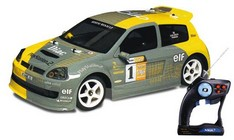
\includegraphics[scale=0.8]{images/renaultclio.jpg}
	\end{center}
	\caption{Renault Clio Rallye 1/10\ieme} 
	\label{renaultclio}
\end{figure}

			
			\subsubsection{Pont en H}
			Nous avons présenté le principe du pont en H à la section précédente.  Nous avons choisi le composant L298 de STMicroelectronics, qui est un double pont en H intégré, à base de transistors bipolaires.
Ce composant permet de contrôler deux moteurs avec un courant de 2A par pont au maximum, ou un seul moteur avec un courant maximum de 4A en utilisant les deux ponts en parallèle. Étant donné les besoin du moteur que nous utilisons, nous avons choisi d’utiliser les deux ponts en parallèle pour contrôler la voiture.
Le pont est activé à l’aide de signaux PWM dont le rapport cyclique D défini la tension moyenne appliquée au moteur : $VMOY = VCC * D$. Le choix de la fréquence est arbitraire, mais peut dépendre de divers paramètres : type de moteur, bruit audible généré, pertes ohmiques.
Enfin, il ne nécessite aucun paramétrage et donc aucun autre composant que les diodes de roue libre. Pour être efficaces, ces diodes doivent être rapides et avoir une tension de seuil très faible : on utilise des diodes Schottky. Elles doivent en outre être capables d’absorber un courant relativement important (quelques ampères), nous avons donc dû commander ces diodes chez Farnell car les diodes disponibles au magasin ne remplissaient pas toutes ces conditions.

\begin{figure}[!h]
	\begin{center}
		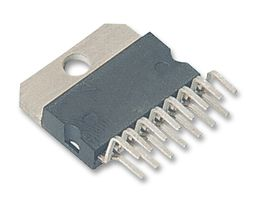
\includegraphics[scale=0.3]{images/L298.jpg}
	\end{center}
	\caption{Un contrôleur L298 de STMicroelectronics} 
	\label{L298}
\end{figure}

			
			\subsubsection{OpenPICUS Flyport}
			Nous avons retenu le module FlyPort de la société OpenPicus. Il s’agit d’un microcontrôleur (PIC24) programmable en langage C, associé à un module Wi-Fi. Cette solution 2-en-1 présente de nombreux avantages. Les fonctions classiques de microcontrôleur nous permettent de générer les signaux PWM nécessaires au contrôle du servomoteur et du pont en H. D’autre part, l’intégration du Wi-Fi nous évite des soucis d’interfaçage avec un module externe, tout en rendant l’ensemble plus compact, plus économe et donc plus facilement intégrale dans notre système.
Notons que ce module ainsi que les logiciels qu’il utilise sont libres et est fourni avec une bibliothèque de fonctions de haut niveau qui nous ont permis de gérer la connexion Wi-Fi  très facilement, notamment en implémentant un serveur TCP. Le logiciel télécommande communique avec le Flyport grâce à un tunnel TCP/IP dans lequel on envoie les commandes sous forme de chaînes de caractères. Le protocole de commande est décrit dans le tableau~\ref{tableaucommandes}.

\begin{figure}[!h]
	\begin{center}
		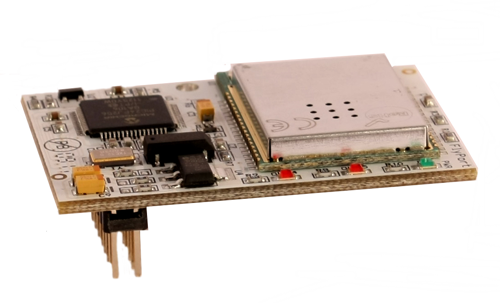
\includegraphics[scale=0.3]{images/flyport.png}
	\end{center}
	\caption{Le Flyport Wi-Fi d'OpenPICUS} 
	\label{flyport}
\end{figure}

\begin{figure}[!h]
	\small
	\begin{center}
		\begin{tabular}{|l|l|l|l|}
		\hline
		\texttt{} \footnotesize\bf{Commande} & \footnotesize\bf{Description} \\ \hline
			\texttt{} A[0-100]  & Avancer avec une puissance donnée entre 0 et 100. \\ \hline
			\texttt{} R[0-100]  & Reculer avec une puissance donnée entre 0 et 100. \\ \hline
			\texttt{} T[0-1000]  & Tourner les roues avant de 0 (gauche) à 1000 (droite). \\ \hline
			\texttt{} S  & Arrêter le moteur de propulsion. \\ \hline
		\end{tabular}
	\end{center}
	\caption{Protocole de commande de la voiture} 
	\label{tableaucommandes}
\end{figure}

\begin{figure}[!h]
	\begin{center}
		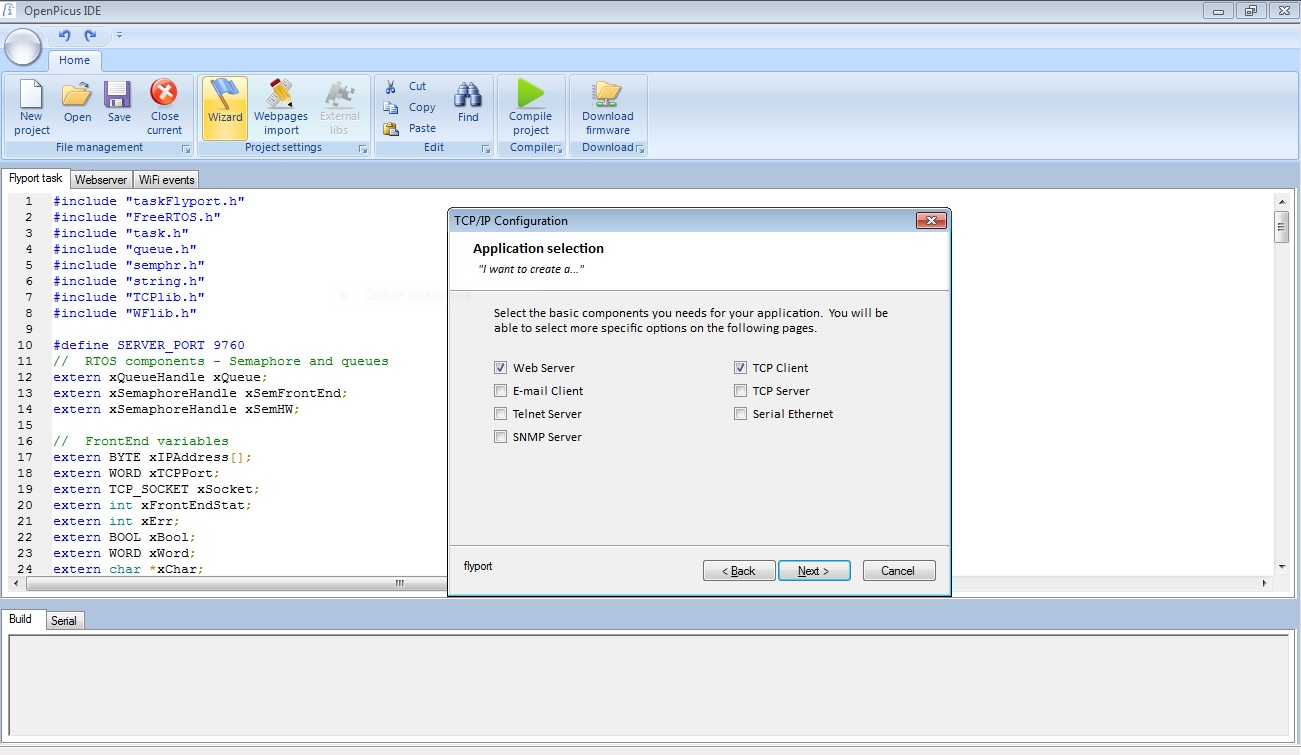
\includegraphics[scale=0.3]{images/openpicus.jpg}
	\end{center}
	\caption{L'environnement de développement OpenPICUS} 
	\label{openpicus}
\end{figure}
			
			\subsubsection{Limitation de courant}
			Un des problèmes auxquels nous avons dû faire face  au cours du projet était de réussir à limiter le courant qui passe dans le moteur. En effet, le contrôleur L298 admet un courant maximal de 4A dans la configuration choisie. Or, lorsque la voiture avance à vive allure ou quand elle est bloquée contre un mur, le courant qui traverse le moteur peut rapidement augmenter à plus de 10A.
Nous n’avons pas réussi à trouver un montage simple à placer sur l’alimentation (VCC) pour directement  limiter le courant. La solution que nous avons retenue est de mesurer le courant du moteur à l’aide d’un résistance, et de désactiver le pont en H lorsque le courant le traversant devient trop important. Le schéma de principe figure~\ref{limitationcourant} illustre le montage.

\begin{figure}[!h]
	\begin{center}
		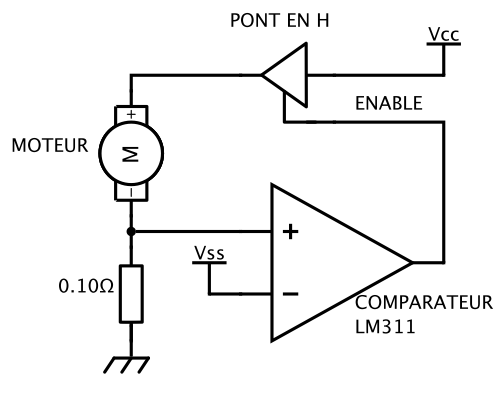
\includegraphics[scale=1]{images/limitationcourant.png}
	\end{center}
	\caption{Limitation du courant du pont en H} 
	\label{limitationcourant}
\end{figure}

La résistance doit avoir une très faible valeur car le courant moyen est de l’ordre de quelques ampères et il faut éviter de dissiper trop de chaleur (donc d’énergie) pour rien. Par ailleurs, le fait que cette résistance soit de type bobinée permet de lisser le courant autour de sa valeur moyenne.
La tension de cette résistance est alors comparée à une tension de référence (VSS) réglée au potentiomètre. Si elle dépasse cette valeur, on désactive le pont en H, ce qui stoppe le courant. On est ainsi certains de ne pas griller le pont en H.
			
			\subsubsection{Alimentation}
			Comme nous l’avons vu précédemment, nous avons décidé de récupérer la batterie de la voiture Nikko. Celle-ci sert d’alimentation au moteur ainsi qu’au servomoteur. A noter que le servomoteur doit être alimenté en +5V et non +7.2V (tension de notre batterie). Nous avons donc choisi d’utiliser un régulateur de tension : le L7805.
D’autre part, le Flyport ainsi que tous les composants logiques nécessitent également une alimentation 5V. Toutefois, il plus sûr de séparer cette alimentation de celles des moteurs car l’utilisation des moteurs créé une chute de tension. Pour cette partie, nous avons donc opté pour une pile 9V couplée à un second régulateur L7805.
			
		\subsection{Réalisation des  PCB}
		Nous avons opté pour une approche de développement incrémental, en commençant par tester le fonctionnement de chaque composant sur plaque à trous en nous aidant de la documentation constructeur, ce qui nous a permis de dimensionner l’ensemble puis de réaliser un prototype, que l’on a amélioré au fur et à mesure du projet.
		
			\subsubsection{Tests préalables}
			Nous avons testé les branchements et le fonctionnement du double pont en H (L298), d’abord sur une résistance de charge, puis sur le moteur lui-même, ce qui nous a permis d’évaluer la puissance dissipée par le pont pour dimensionner son radiateur. Avec du recul, nous nous sommes rendus compte que nous avions probablement endommagé le pont pendant cette phase de tests et qu’il chauffait anormalement ; nous l’avons donc remplacé. Nous avions ainsi choisi le radiateur pour qu’il permette de dissiper 10 Watts, ce qui est largement supérieur à ce qui est en fait nécessaire. Ce test a également permis de valider le choix de la résistance de \unit{100}{\milli \ohm} pour la mesure du courant traversant le moteur.
Une fois le fonctionnement du pont validé, nous avons testé le fonctionnement du comparateur de tension (LM311), servant à désactiver le pont en H dès que le courant le traversant devient trop élevé.
Parallèlement, nous avons testé la génération de signaux PWM à l’aide du Flyport avec l’oscilloscope, ainsi que la connexion Wi-Fi, pour finir par une série de tests avec le reste du montage sur plaque à trous.
			
			\subsubsection{Design et test des circuits imprimés}
			Nous avons décidé de séparer la partie logique comprenant le Flyport de la partie puissance comprenant le L298, afin de faciliter les révisions et de séparer partie commande et partie opérative. En outre, cette séparation protège la partie logique (tensions et courants faibles) d’éventuelles défaillances de la partie puissance (tensions et courants élevés).
			
				\paragraph{Version 1}
				Le premier prototype du circuit a été réalisé et routé sous Altium. Il nous a permis de tester le fonctionnement de la voiture et d’avancer sur la programmation du microcontrôleur et des programmes pour le télécommander.
Cette première version a permis de mettre en évidence plusieurs manques :
\begin{itemize}
\item Les deux cartes n’étaient maintenues ensemble que par un connecteur rigide. Étant donnée la masse du radiateur utilisé, elles étaient susceptibles de se dissocier en marche. Ceci a été corrigé par la réalisation d’un support temporaire en plexiglas.
\item Le dissipateur du L298 n’était fixé qu’au composant et appuyait sur ses connexions.
\item Certaines pistes de la partie puissance ne sont pas assez larges : l’une d’entre elles s’est décollée à cause de la chaleur dissipée par le L298 défectueux.
\item La résistance de \unit{100}{\milli \ohm} est trop proche du L298, ce qui fait parfois fondre ses soudures.
\item Certaines soudures étaient difficiles à réaliser, car les pads prévus étaient trop petits.
\item Le connecteur rigide entre les deux cartes était peu pratique à brancher.
\item Un des deux régulateurs de tension sur la partie commande est trop proche du Flyport, ce qui gêne pour placer son dissipateur.
\end{itemize}


				\paragraph{Version 2}
				La version 2 du circuit imprimé corrige tous les problèmes de la version précédente :
\begin{itemize}
\item Des emplacements pour visser les deux cartes ont été réalisés. Les deux cartes sont désormais vissées ensemble, et reliées par une nappe souple qui se branche / débranche aisément.
\item Le dissipateur du L298 repose sur une vis et de la placea été prévue de chaque côté de la carte pour le visser.
\item Toutes les pistes de la partie puissance ont été élargies (80 mil minimum) et étamées.
\item Les composants ont été écartés les uns des autres afin de limiter leur échauffement.
\end{itemize}
Le pont L298 est un composant classique, facile à utiliser et peu onéreux. Cependant, il a l’inconvénient de chauffer beaucoup. Afin de le remplacer par un composant plus performant, une carte utilisant un composant de surface (VNH3SP30 de STMicroelectronics) a été proposée.

\begin{figure}[!h]
	\begin{center}
		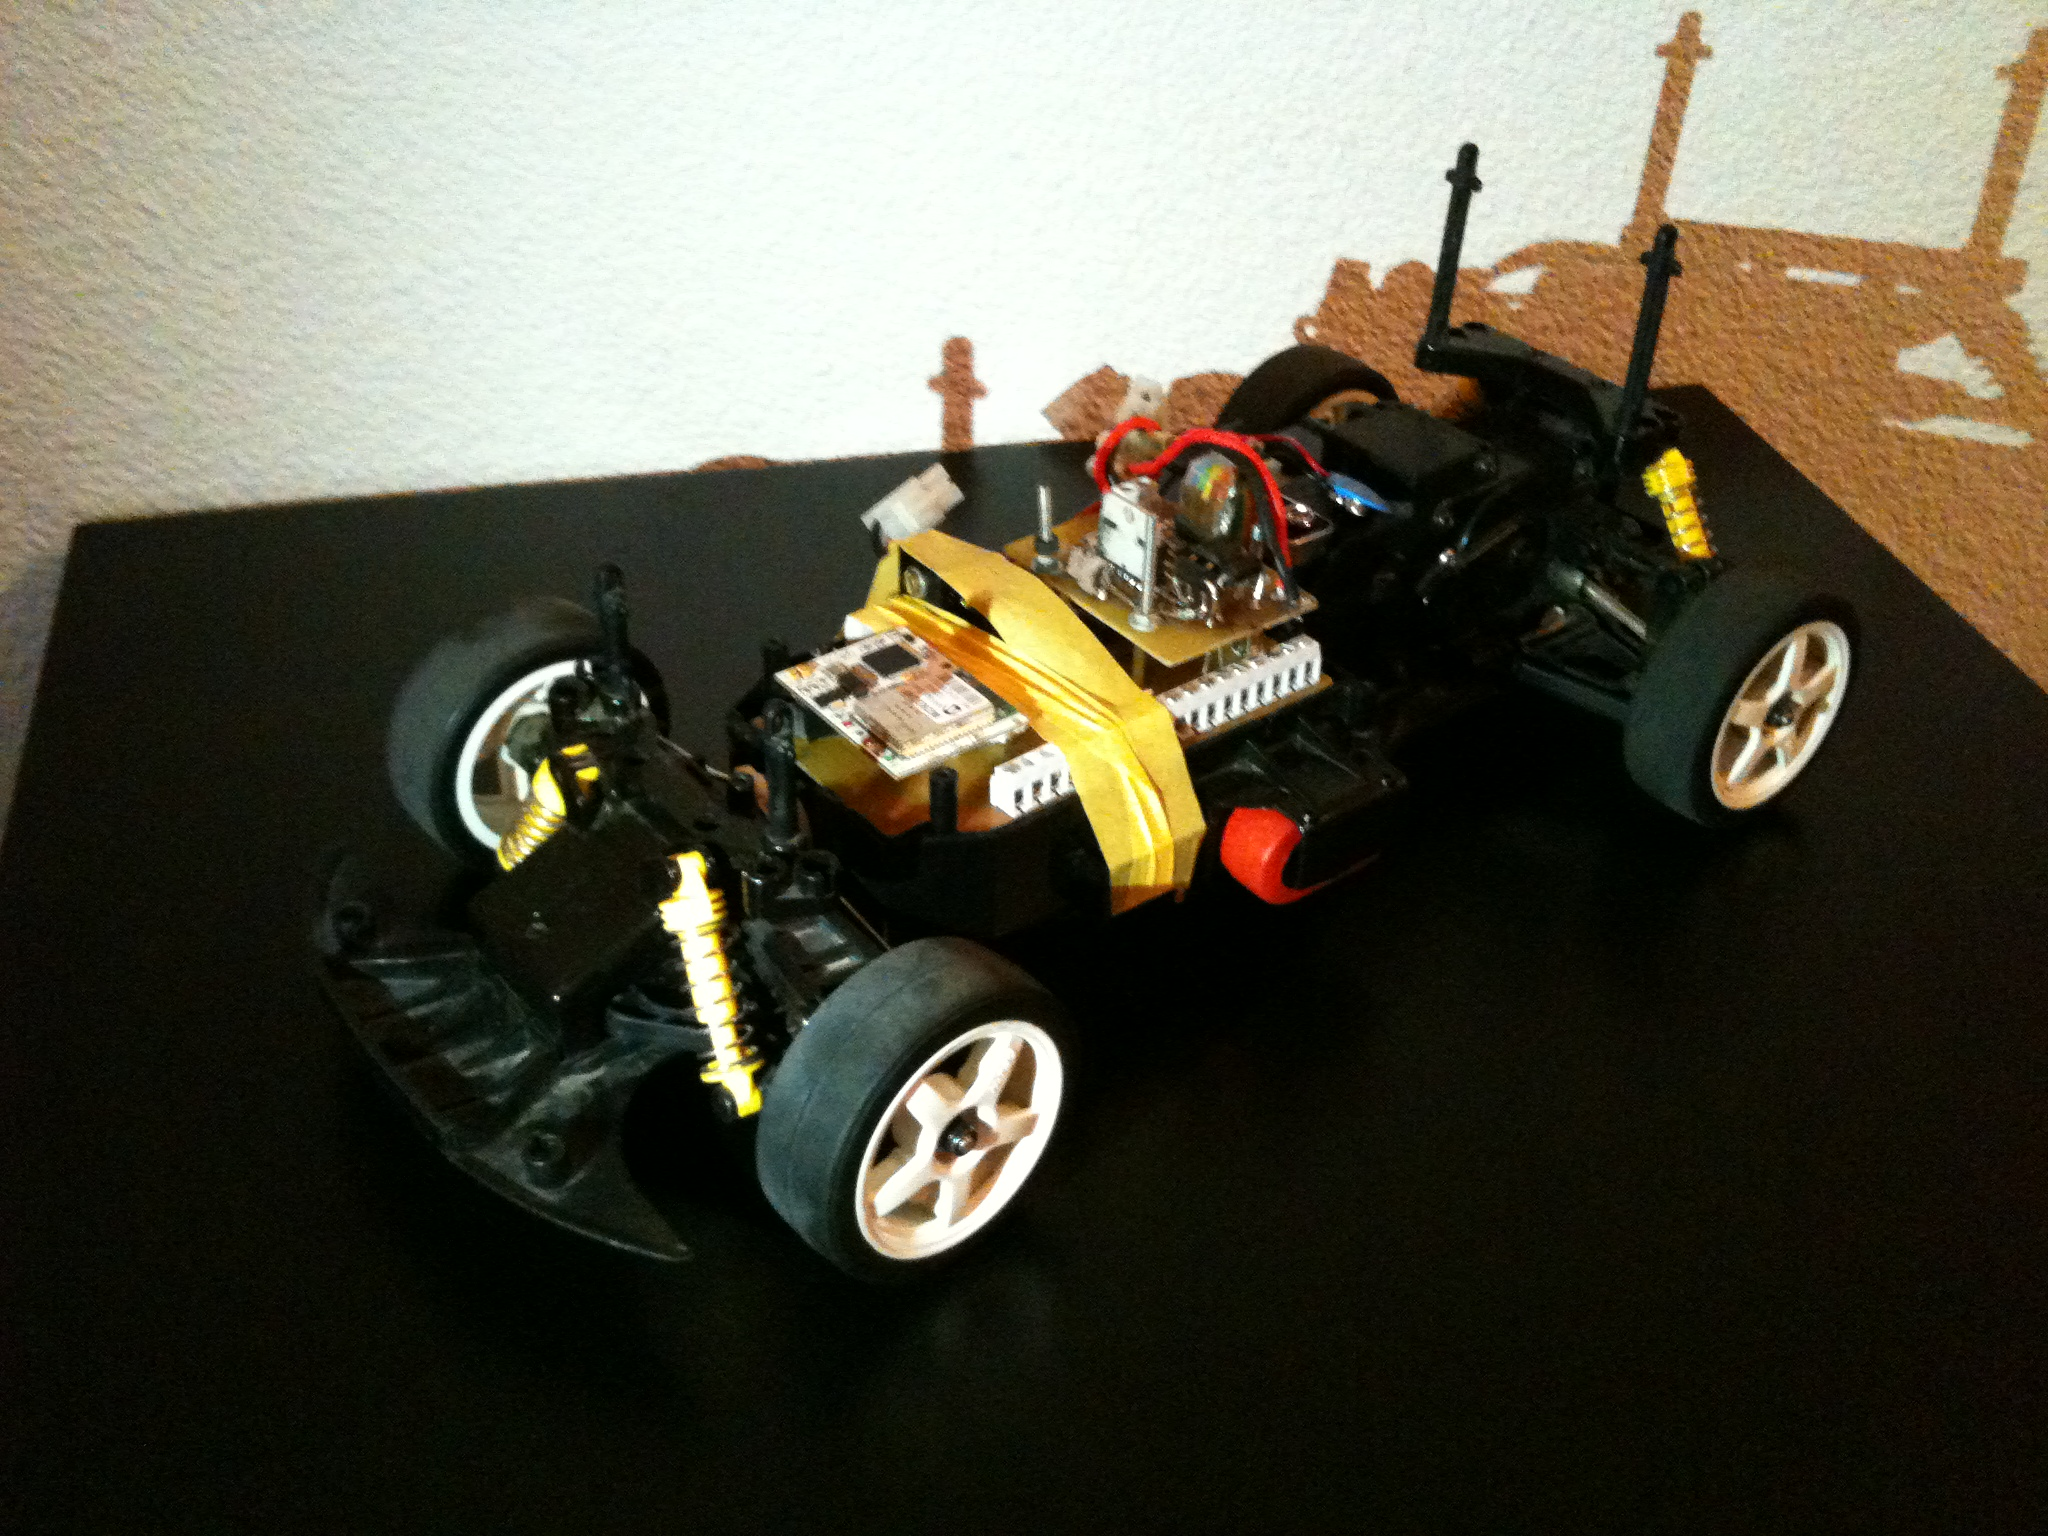
\includegraphics[scale=0.22]{images/voiture.jpg}
	\end{center}
	\caption{La voiture avec les deux cartes superposées} 
	\label{voiture}q
\end{figure}
		
		\subsection{Logiciel de commande	}
		Nous avons décidé de retenir deux plateformes distinctes : un ordinateur et un smartphone sous Android.
		
			\subsubsection{Ordinateur}
			Il est ici nécessaire d’utiliser une bibliothèque graphique. Au vu de la variété des environnements de développement des personnes travaillant sur ce projet (Windows / Mac / Linux), la solution se devait d’être multi-plateforme, c’est-à-dire que le même code source devrait pouvoir être compilé et exécuté sur toutes les machines. De plus, pour des raisons de coût, la licence doit être gratuite. Plusieurs solutions existent en la matière, les deux plus répandues étant Qt et WxWidget. Toutes les deux nécessitent d’utiliser le langage C++. Nous avons décidé de retenir Qt pour sa documentation plus large et sa plus grande communauté d’utilisateurs.
Un rendu visuel de l’application Windows est fournie figure~\ref{logicielqt}. %Pour les sources, on renvoie le lecteur à l’annexe XXX

\begin{figure}[!h]
	\begin{center}
		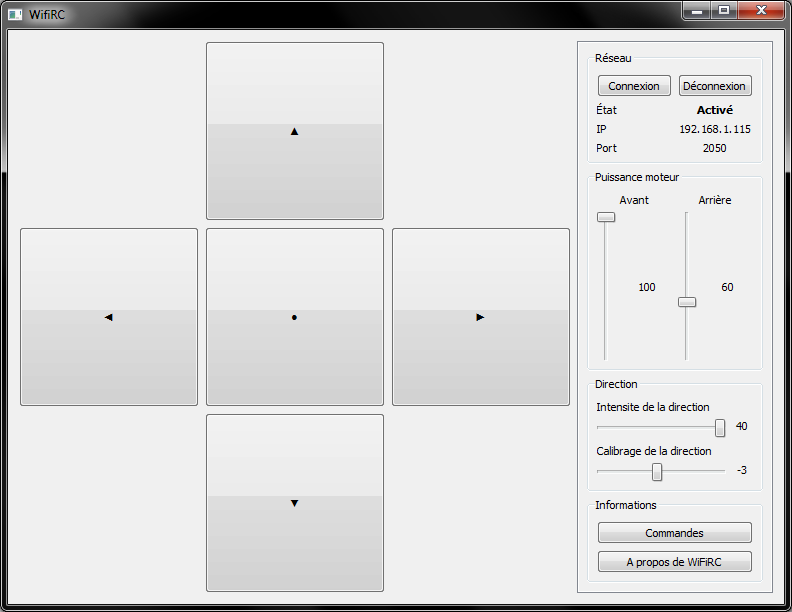
\includegraphics[scale=0.4]{images/logicielqt.png}
	\end{center}
	\caption{Le logiciel de contrôle développé sous Qt} 
	\label{logicielqt}
\end{figure}

			\subsubsection{Smartphone}
			Ici, la priorité était de réaliser une interface conviviale permettant à l’utilisateur un contrôle rapide et facile de la voiture. Un problème demeurait : sur quel OS travailler ? On s’aperçoit qu’Android et iOS équipent plus de la moitié des terminaux mobiles. Toutefois, un développement pour iOS demeure trop contraignant : il nécessite de posséder un Mac et surtout un compte développeur payant. Le développement pour Android nécessite quant à lui l’utilisation du langage Java.
Nous avons donc décidé de retenir la plateforme Android. Son rendu visuel est fourni figure~\ref{logicielandroid}. % et son code source en annexe XXX.

\begin{figure}[!h]
	\begin{center}
		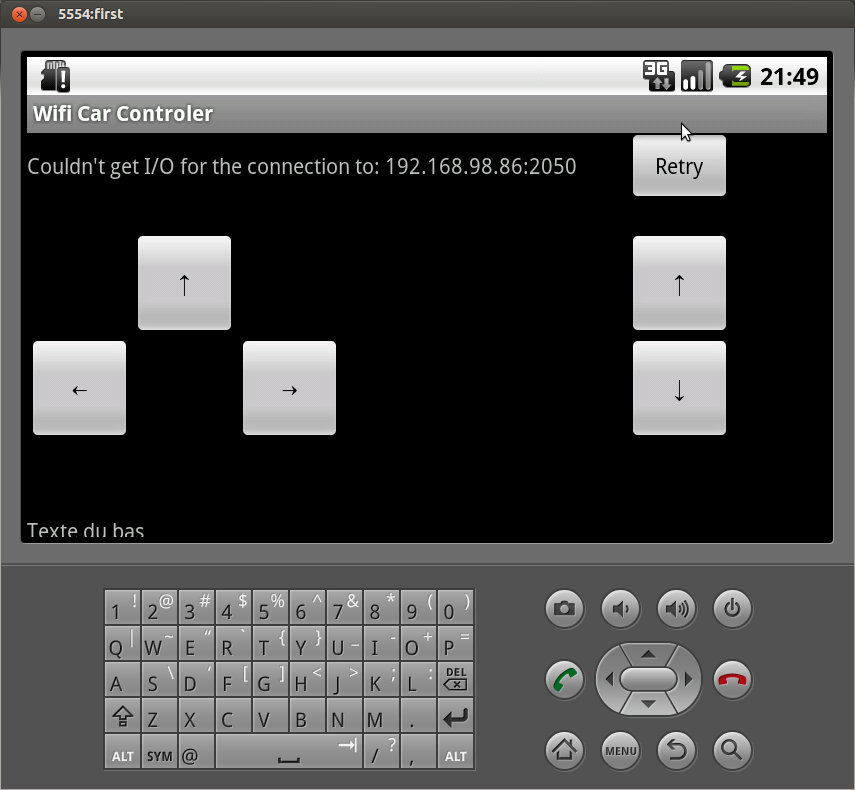
\includegraphics[scale=0.4]{images/logicielandroid.png}
	\end{center}
	\caption{Le logiciel de contrôle développé sous Android} 
	\label{logicielandroid}
\end{figure}

			Personne n’étant très compétent en Java, l'application Android a été réduite au minimum : des boutons pour contrôler la direction et la propulsion. Néanmoins il reste toujours la possibilité d’implémenter la gestion de l'accéléromètre du smartphone pour diriger la voiture.
A l’heure de la rédaction de ce rapport, un problème demeure. Le Wi-Fi intégré à Android ne permet que la connexion à des réseaux de type Infrastructure. Même s’il est en théorie possible pour le FlyPort de se connecter à des réseaux de ce type, nos derniers essais se sont soldés par des échecs. On espère trouver l’origine de ce problème lors de notre dernière séance de projet afin de proposer une démonstration un peu plus ludique de notre projet lors des présentations.

	\section{Tests finaux}
	Une fois l’ensemble terminé, nous avons procédé à quelques tests pour connaître les performances du système et voir si celles-ci correspondent bien à ce à quoi nous nous attendions.
	
		\subsection{Portée de la voiture}
		 Le Flyport comporte un module Wi-Fi (MicroChip MRF24WB0MB) dont la documentation indique une portée pouvant aller jusqu’à 400 mètres en champ libre. Nous avons de notre coté testé la réception à une distance de 100 mètres en champ libre sans le moindre problème. Il serait intéressant de faire des essais à des distances plus grandes pour connaître la portée réelle de la voiture.
		
		\subsection{Autonomie}
		Il s’agit là d’un des principaux défauts du Wi-Fi. Ce protocole étant assez haut niveau, il est par nature beaucoup plus gourmand qu’une radio-transmission classique. Ceci explique que ce type de transmission ne soit pas devenue, même à l’ère du tout-numérique, la norme en matière de radiomodélisme. Une mesure avec le Wi-Fi en fonctionnement réalisée avec une alimentation externe montre que le système consomme environ 150 mA au repos avec le Wi-Fi activé.
En pratique, ceci permet d’obtenir une autonomie variant entre 30 et 45 minutes pour la partie logique avant que la batterie ne doive être rechargée. A noter toutefois qu’aucune démarche réelle d’économie d’énergie (hormis le choix du FlyPort) n’a été faite tant sur le plan matériel que logiciel. Ces valeurs pourraient donc être améliorées moyennant quelques efforts supplémentaires.
	La batterie qui alimente les moteurs présente quant à elle une autonomie de 15 à 30 minutes selon l’utilisation, ce qui est conforme à l’autonomie d’origine de la voiture. Ceci est plutôt rassurant car cela montre qu’il n’y a pas plus de pertes d’énergie qu’avec l’électronique d’origine.
		
		\subsection{Choix des paramètres moteurs}
		Les derniers tests que nous avons effectués se sont portés sur l’optimisation des paramètres moteurs. En tête de liste, on trouve le réglage de la fréquence du PWM de commande du moteur DC. Des essais avec des fréquences de 500 Hz et 10 kHz se sont révélés concluants sur le plan du fonctionnement, mais gênants en terme de bruit, la première provoquant un son grave en fonctionnement et la seconde un son aigu. Nous avons donc décidé de choisir une fréquence quasi inaudible pour l’oreille humaine : 20 kHz. Avec ce choix, aucun bruit désagréable ne ressort de l’utilisation du moteur et le comportement général ne semble pas pour autant altéré.



\chapter{Gestion de projet}

	\section{Aspects organisationnels}
	Afin de partager les informations nous avons utilisé un service de partage de documents et de travail collaboratif : Google Documents, pour sa facilité d’utilisation. Nous l’utilisons notamment en tant que carnet de bord pour noter en fin de séance ce qui a été réalisé, les difficultés rencontrées et le travail à réaliser pour la séance suivante. Il contient également tous les documents importants concernant le projet.
Nous avons également mis en place un espace sur Google Code, qui contient tout les codes des programmes réalisés ainsi que diverses information sur le projet. Il permet d’utiliser un logiciel de gestion de versions (SVN), un wiki contenant des informations sur les différentes parties du projet, ainsi que des explications de codes.

Le site est accessible à l’adresse suivante : \href{http://code.google.com/p/flyport-wifi-rc-car/}{http://code.google.com/p/flyport-wifi-rc-car/}.
	
	\section{Diagramme de Gant}
	Le découpage du système et l’analyse des besoins nous a permis d’identifier un certain nombre de tâches à effectuer dans le cadre du projet. Nous les avons regroupées dans un diagramme de Gantt (en annexe~\ref{gantt}) qui a été réalisé en début de projet (mois de janvier). Nous avions prévu du temps en fin de projet pour réaliser le rapport final, le support de communication ainsi que les différents «bonus» (application smartphone, caméra, capteurs).
Malheureusement, il semble que nous ayons été trop optimistes : en effet, les différents problèmes rencontrés nous ont beaucoup retardés. Nous avons passé plus de temps que prévu sur certains points, notamment sur la partie électronique que nous avons dû revoir.

	\section{Gestion financière}
	La gestion financière du projet a été relativement simple, car bien que le matériel nécessaire ait un certain coût, nous n’avons pas eu à payer la plupart des éléments. En effet, nous avons récupéré une voiture radio-commandée appartement à un des membres du groupe, et le magasin d’électronique de l’école disposait de la plupart des choses dont nous avions besoin. Le Flyport nous a été gracieusement offert par la société OpenPICUS, et le pont en H (L298) par STMicroelectronics.
	Le tableau~\ref{tableaumateriel} rassemble tous les éléments matériels nécessaires à la réalisation du projet.
	
\begin{figure}[!h]
	\scriptsize
	\begin{center}
		\begin{tabular}{|l|l|l|l|l|}
		\hline
		\texttt{} \scriptsize\bf{Désignation} & \scriptsize\bf{Fournisseur / Fabriquant} & \scriptsize\bf{P.U.H.T. (\euro)} & \scriptsize\bf{Qté} & \scriptsize\bf{Total TTC (\euro)} \\ \hline
			\texttt{} Flyport Wi-Fi & OpenPicus & 49 \euro & 1 & 58,60 \\ \hline
			\texttt{} Voiture R/C de récupération & Nikko R/C 1/10\ieme & 16,72 \euro & 1 & 20,00 \\ \hline
			\texttt{} Servomoteur HS-422 & HiTec / Magasin d’Électronique & 8,9 \euro & 1 & 10,64 \\ \hline
			\texttt{} PCBs Logique et puissance & Réalisé à l’école & 4,18 \euro & 1 & 5,00 \\ \hline
			\texttt{} Comparateur LM311 & STMicroelectronics / Magasin & 0,25 \euro & 1 & 0,30 \\ \hline
			\texttt{} Potentiomètre 10K\ohm & Magasin d’Électronique & 0,32 \euro & 1 & 0,39 \\ \hline
			\texttt{} Régulateur L7805 & Magasin d’Électronique & 0,31 \euro & 2 & 0,74 \\ \hline
			\texttt{} Bouton poussoir & Magasin d’Électronique & 0,34 \euro & 1 & 0,40 \\ \hline
			\texttt{} Résistances, capacités, LED & Magasin d’Électronique & 0,84 \euro & 1 & 1,00 \\ \hline
			\texttt{} Contrôlleur L298 & STMicroelectronics & 6,26 \euro & 1 & 7,49 \\ \hline
			\texttt{} Résistance bobinée 0.1\ohm 5W & Magasin d’Électronique & 1,59 \euro & 1 & 1,90 \\ \hline
			\texttt{} Diodes Schottky & Farnell / Fairchild Semi & 0,52 \euro & 4 & 2,49 \\ \hline
			\texttt{} Dissipateur thermique & Magasin d’Électronique & 0,50 \euro & 1 & 0,60 \\ \hline
		 \scriptsize\bf{Total TTC (\euro)} & \multicolumn{4}{c|}{ \scriptsize\bf{109,55 \euro}} \\ \hline
	\end{tabular}
	\end{center}
	\caption{Protocole de commande de la voiture} 
	\label{tableaumateriel}
\end{figure}
	
	\section{Retours personnels de projet}
	
	\paragraph{Florian Castellane}
	Le projet de groupe aura été très formateur pour moi car il a permis de voir le processus complet de développement : le produit fini est différent de ce qui a été pensé initialement, avec des bonnes surprises comme des déceptions parfois. Je pense notamment à notre volonté d’avoir un retour vidéo de la voiture, qui pourrait finalement être l’objet d’un sujet de projet à elle seule pour pouvoir être implémentée sur notre matériel. D’ailleurs, ce projet, je pense, est assez intéressant pour être amélioré lors de futurs projets de groupe à Phelma. Mais le plus intéressant a été le nombre de compétences dont il a été possible de tirer partie lors du projet: nous avons fait de l’électronique et de la programmation bien sûr, mais aussi de la mécanique, des calculs pour dimensionner le refroidissement du driver du moteur, de la gestion du groupe et du temps de travail, des connaissances en informatique sur le travail collaboratif... Pour finalement conduire une voiture radiocommandée par Wi-Fi !
	
	\paragraph{Guillaume Mahieux}
	Ce projet a été une bonne expérience de travail en groupe car chacun a participé à la bonne ambiance et à la cohésion du groupe. C’était un projet motivant car il a un coté ludique, tout en mettant en œuvre des domaines variés et qui nous intéressaient tous. Il a été l’occasion d’approfondir nos compétences en électronique (Pont en H, limitation de courant, PWM), en programmation (C sur le Flyport, C++ pour Qt et Java pour Android) et d’apprendre à concevoir puis améliorer un système complet à l’aide de technologies sans fil. Je pense que ce projet a été déterminant dans ma vision des différentes filières proposées par l’école et dans les choix que j’ai effectué pour l’année prochaine.
	
	\paragraph{Jérémy Fanguede}
	Ce projet aura été dans l’ensemble plus que bénéfique. Il m’aura permis de me familiariser avec la programmation sur microcontrôleur ainsi qu’au fonctionnement des réseaux, notamment Wi-Fi. Il aura été l’occasion d’améliorer certaines de mes compétences, plus particulièrement la conception de cartes électroniques, ainsi que la programmation d’interfaces graphiques (sur PC et smartphone).
Le projet a été intéressant jusqu’à la fin, d’autant plus qu’il touché deux domaines qui m’intéressent tout particulièrement ; l’électronique et l’informatique. Il m’a aussi permis de me rendre compte à quel point les aspects “travail en groupe et gestion de projet” étaient  important, notamment pour le respect des calendriers.
	
	\paragraph{Tavares Florian}
	Je garderai une très bonne expérience de ce projet de groupe. Il m’a permis de me rendre compte des avantages et des inconvénients du travail collectif. Sur le plan du sujet, il a su attiser ma curiosité en alternant les aspects techniques et ludiques et en touchant à des domaines que j’affectionne tout particulièrement : la micro-électronique et le développement logiciel.
Un autre bon point à noter : au départ du projet, chacun des membres du groupe est arrivé avec son bagage de compétences techniques, ses points faibles et ses points forts. Il me semble qu’au bout de ses quelques mois, ces disparités ont disparu (dans le bon sens bien sûr !). Chacun de nous pourrait aborder de manière indépendante chacune des différentes parties du projet sur la plan technique ce qui était loin d’être le cas au début !
Ce projet m’aura également permis de me rendre compte que la gestion d’un planning peut parfois relever du parcours du combattant. Sur le plan pratique, je retiendrai l’utilisation de nombreux outils de travail collaboratif (type Google Docs, Google Code) facilitant grandement la productivité en groupe.
	

\chapter{Conclusion}
Avant tout, le projet a beaucoup appris à chacun d’entre nous. Ainsi, alors que nous disposions de compétences spécifiques très différentes, nous avons su nous organiser pour en tirer le maximum tout en apprenant nos compétences au groupe, et en nous perfectionnant.
Au terme de ce Projet de Groupe, nous disposons d’un modèle fonctionnel de voiture télécommandée par Wi-Fi, et dont l’utilisation est à la fois simple et ludique. Toutefois, notre système est encore perfectible et des idées d’améliorations nous ont traversé l’esprit. On pense notamment à:
\begin{itemize}
\item l’implémentation d’un retour vidéo de la voiture,
\item l’installation de capteurs (rendue possible par le microcontrôleur utilisé),
\end{itemize}

Ces idées pourraient d’ailleurs constituer la base de futurs projets de robotique et rendraient notre système plus autonome et/ou plus polyvalent.

\chapter{Annexes}

\begin{sidewaysfigure}
\centering
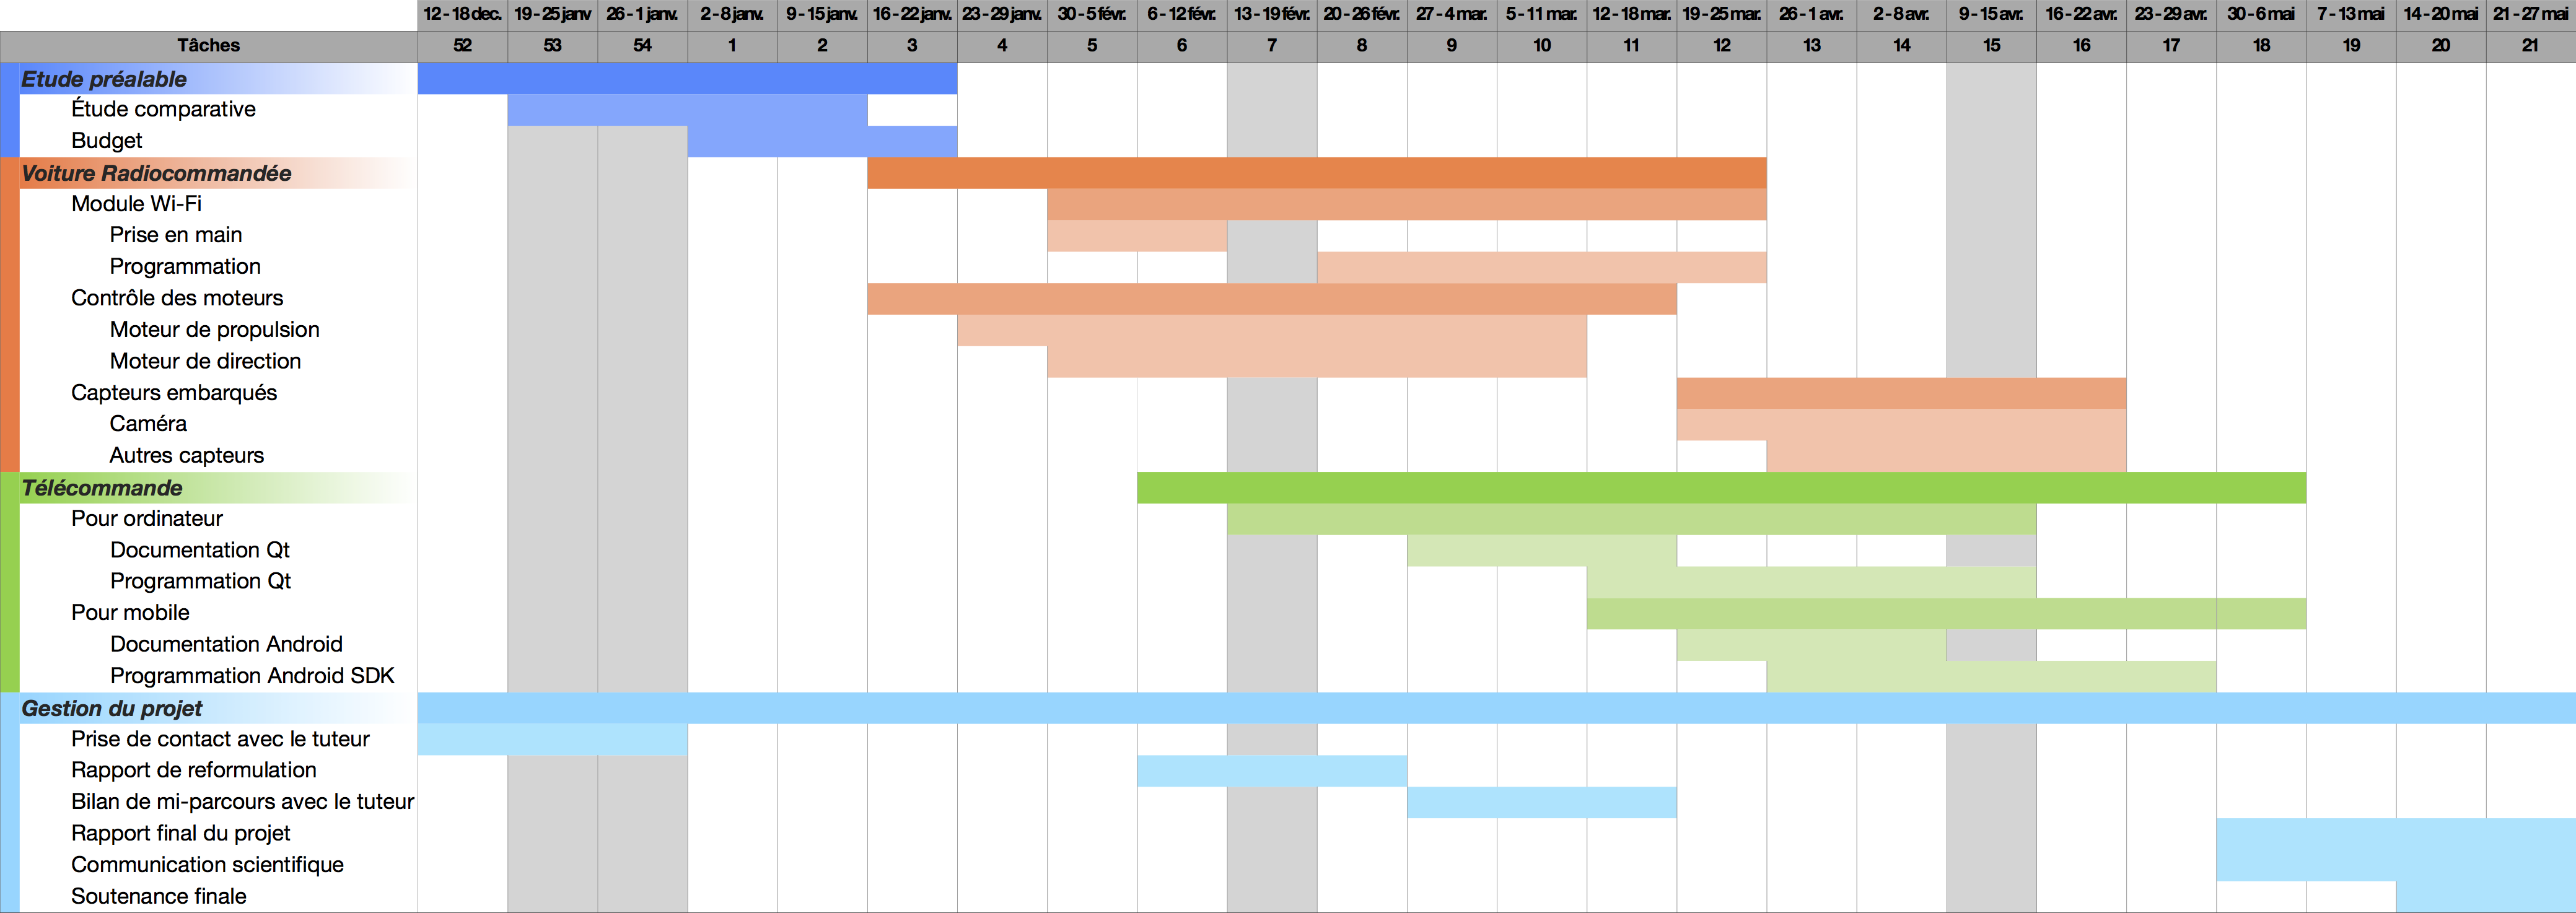
\includegraphics[scale=0.35]{images/gantt.png}
\caption{Diagramme de GANTT}
\label{gantt}
\end{sidewaysfigure}

\end{document}
